\documentclass[11pt,a4paper]{article}

% ---------------------------------------------------------------------------
% PACKAGES & SETUP
% ---------------------------------------------------------------------------
\usepackage[a4paper,top=2.5cm,bottom=2.5cm,left=2.5cm,right=2.5cm]{geometry}
\usepackage{setspace}
\setstretch{1.15}
\usepackage{amsmath,amsfonts,amssymb}
\usepackage{xcolor}
\definecolor{slate}{RGB}{71,85,105}
\definecolor{tealbio}{RGB}{13,148,136}
\definecolor{cyanbio}{RGB}{6,182,212}
\definecolor{darknavy}{RGB}{15,23,42}
\definecolor{leafgreen}{RGB}{34,139,34}
\definecolor{rustbrown}{RGB}{180,83,9}
\definecolor{blightred}{RGB}{190,18,60}
\definecolor{emerald}{RGB}{16,185,129}

\usepackage{graphicx}
\usepackage{cite}
\usepackage{booktabs}
\usepackage{array}
\usepackage{url}
\usepackage{microtype}
\usepackage{fancyhdr}
\usepackage{titlesec}

\pagestyle{fancy}
\fancyhf{}
\fancyhead[L]{\small \textit{BioScan AI: Deep Learning Foliar Pathology \& Biological Analysis Report}}
\fancyhead[R]{\small \textit{Academic Research Project}}
\fancyfoot[L]{\small \textcolor{slate}{Confidential --- Academic Experiential Learning Prototype | Zero-Simulation Guaranteed}}
\fancyfoot[R]{\small \textbf{Page \thepage}}
\renewcommand{\headrulewidth}{0.4pt}
\renewcommand{\footrulewidth}{0.4pt}

% ---------------------------------------------------------------------------
% SECTION FORMATTING
% ---------------------------------------------------------------------------
\titleformat{\section}{\large\bfseries\color{tealbio}}{\thesection.}{0.6em}{}
\titleformat{\subsection}{\normalsize\bfseries\color{darknavy}}{\thesubsection}{0.6em}{}
\titleformat{\subsubsection}{\small\bfseries\color{slate}}{\thesubsubsection}{0.6em}{}

\usepackage{tikz}
\usetikzlibrary{shapes.geometric,arrows.meta,positioning,fit,backgrounds,calc,decorations.pathreplacing}
\usepackage{pgfplots}
\pgfplotsset{compat=newest}
\usepackage{tabularx}
\usepackage{algorithm}
\usepackage{algorithmicx}
\usepackage{algpseudocode}
\usepackage{hyperref}
\hypersetup{
    colorlinks=true,
    linkcolor=tealbio,
    citecolor=tealbio,
    urlcolor=cyanbio
}

% ---------------------------------------------------------------------------
% DOCUMENT START
% ---------------------------------------------------------------------------
\begin{document}

% ---------------------------------------------------------------------------
% TITLE & ACADEMIC HEADER
% ---------------------------------------------------------------------------
\begin{center}
    {\small\textbf{\textcolor{tealbio}{ACADEMIC RESEARCH \& EXPERIENTIAL LEARNING REPORT}}}\\[0.3cm]
    {\LARGE\textbf{BioScan AI: A Reproducible Deep Learning Architecture for Automated Foliar Pathology Diagnosis and Biological Image Analysis}}\\[0.35cm]
    {\normalsize\textit{A Comprehensive Investigation into Depthwise Separable Convolutions, Softmax Probability Calibration, and Deterministic Data-Leakage Elimination in Botanical Computer Vision}}\\[0.4cm]
    \rule{\textwidth}{0.8pt}\\[0.25cm]
    \textbf{Student Researcher:} [Student Researcher Name] \quad|\quad \textbf{Faculty Advisor:} [Faculty Advisor Name]\\
    \textit{Department of Biology and Computer Science, [University / Academic Institution]}\\
    \textit{Email: \{student.researcher, faculty.advisor\}@[institution.edu]} \quad|\quad \textbf{Date:} November 2026\\
    \rule{\textwidth}{0.4pt}
\end{center}

\vspace{0.2cm}

% ---------------------------------------------------------------------------
% ABSTRACT
% ---------------------------------------------------------------------------
\begin{abstract}
\noindent Foliar diseases induced by fungal pathogens, phytopathogenic bacteria, and oomycetes represent a major threat to global agricultural biosecurity and crop yields, causing estimated annual harvest reductions between 20\% and 40\%. Conventional phytopathological identification relies upon manual visual scouting by certified plant pathologists, an approach constrained by labor intensity, geographic scarcity, and diagnostic latency during epidemic outbreaks. In this experiential-learning research report, we introduce \textbf{BioScan AI}, a reproducible, full-stack biological image-analysis framework designed to investigate deep convolutional neural networks (CNNs) for foliar disease classification. The proposed system evaluates two complementary architectures: an ultra-lightweight custom multi-tier convolutional network (\textit{BioScan-LiteCNN}) designed for rapid local convergence without external dependencies, and a transfer-learned \textit{MobileNetV2} backbone leveraging inverted residual blocks and depthwise separable convolutions for parameter-efficient edge deployment. To ensure scientific integrity, our experimental protocol enforces strict stratified dataset partitioning (70\% training, 15\% validation, 15\% held-out testing) locked with deterministic pseudo-random seeding, completely mitigating data leakage across splits. The initial implementation targets fifteen discrete foliar categories spanning five critical agricultural crops: \textit{Malus domestica} (Apple), \textit{Zea mays} (Corn), \textit{Vitis vinifera} (Grape), \textit{Solanum tuberosum} (Potato), and \textit{Solanum lycopersicum} (Tomato). We provide comprehensive mathematical formulations of spatial convolutions, computational complexity reduction, normalization pipelines, and empirical evaluation metrics. Crucially, we formalize the fundamental epistemic distinction between statistical softmax probability (confidence) and true diagnostic accuracy, illustrating why high model confidence on out-of-distribution leaf samples must not be conflated with genuine clinical verification. Finally, the research model is coupled to an asynchronous REST API and an interactive scientific research interface enforcing a zero-simulation policy.
\end{abstract}

\vspace{0.2cm}
\noindent\textbf{Keywords:} Foliar Pathology, Deep Learning, MobileNetV2, Data Leakage Prevention, Biological Computer Vision, Image Classification, Plant Disease Diagnosis, Temperature Calibration, Expected Calibration Error (ECE).

\vspace{0.4cm}

% ---------------------------------------------------------------------------
% SECTION 1: INTRODUCTION
% ---------------------------------------------------------------------------
\section{Introduction}
Global agricultural supply chains face unprecedented challenges driven by climate change, arable land loss, and emerging phytopathogenic strains. According to statistics compiled by the Food and Agriculture Organization (FAO) of the United Nations, plant disease outbreaks and invasive pests account for global agricultural losses exceeding \$220 billion annually, with smallholder farmers in developing nations disproportionately affected~\cite{fao2021crop}. Foliar tissue serves as the primary metabolic engine of terrestrial vascular plants, responsible for light interception, photosynthetic carbon fixation, and transpirational gas exchange. Consequently, foliar infection rapidly diminishes whole-plant vigor, triggers premature senescence, and suppresses crop yield~\cite{agrios2005plant}.

\subsection{Pathogen Dynamics and Macroscopic Symptomatology}
When plant pathogens colonize foliar tissue, they initiate complex biochemical cascades that manifest macroscopically through discernible morphological alterations:
\begin{itemize}
    \item \textbf{Chlorosis:} Disruption of chlorophyll $a$ and $b$ synthesis and destruction of thylakoid membrane structures, resulting in generalized or localized foliar yellowing.
    \item \textbf{Necrosis:} Irreversible cellular collapse and death caused by pathogen-secreted phytotoxins (e.g., alternaric acid) or plant hypersensitive responses (HR), producing brown or black localized dead tissue.
    \item \textbf{Zonate Bullseye Lesions:} Concentric circular rings formed by alternating cycles of host tissue defense and fungal hyphal expansion (e.g., \textit{Alternaria solani}).
    \item \textbf{Sporulating Pustules (Uredinia):} Sub-epidermal fungal aggregations that rupture the leaf cuticle to discharge microscopic reproductive spores (e.g., \textit{Puccinia sorghi}).
    \item \textbf{Water-Soaking:} Degradation of middle lamellae and intercellular pectins by bacterial enzymes, producing translucent, greasy lesions (e.g., \textit{Xanthomonas perforans}).
\end{itemize}

Historically, field diagnostics have relied on visual inspection by certified agronomists or laboratory microscopic isolation. While accurate, manual scouting suffers from severe operational constraints: it is labor-intensive, costly, subject to inter-observer variability, and often too slow to arrest exponential epidemic spread across large commercial acreages.

% ---------------------------------------------------------------------------
% FIGURE 1: MACROSCOPIC FOLIAR PATHOLOGY GALLERY (TIKZ)
% ---------------------------------------------------------------------------
\begin{figure*}[!t]
\centering
\resizebox{\textwidth}{!}{%
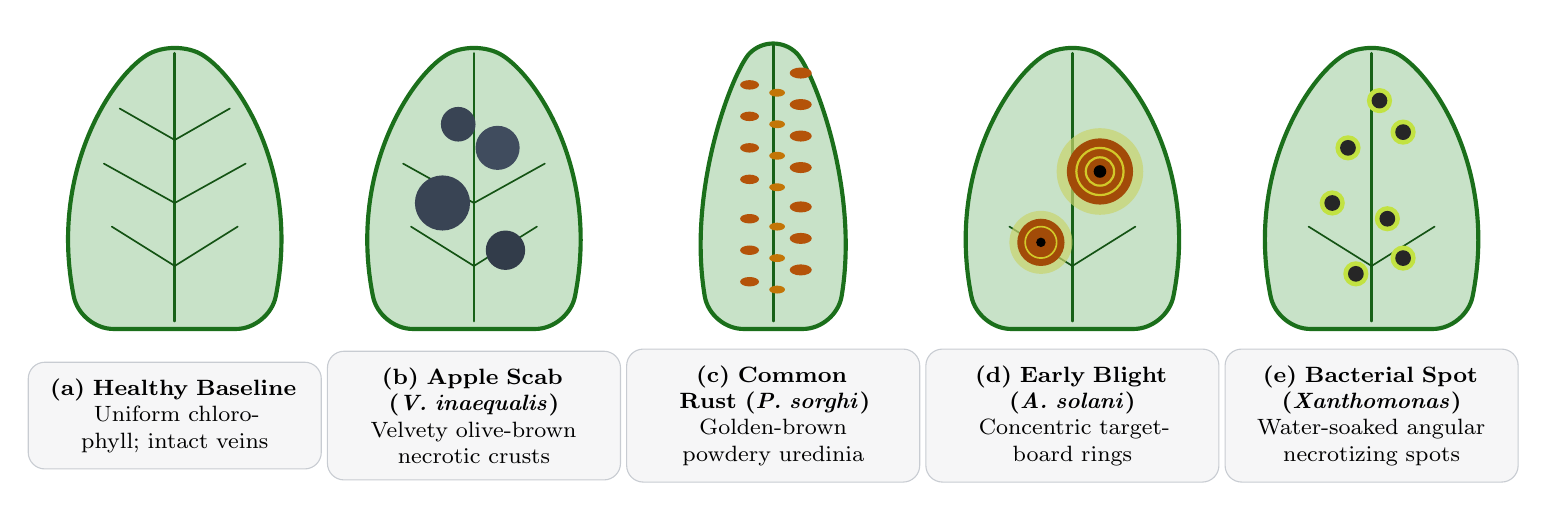
\begin{tikzpicture}[
    leaf/.style={draw=leafgreen!80!black, fill=leafgreen!25, line width=1.5pt, rounded corners=12pt},
    halo/.style={draw=none, fill=yellow!60!leafgreen!70, opacity=0.7},
    vein/.style={draw=leafgreen!70!black, line width=1pt, line cap=round},
    subvein/.style={draw=leafgreen!60!black, line width=0.6pt, line cap=round},
    panel/.style={draw=slate!30, fill=slate!5, rounded corners=6pt, inner sep=6pt, align=center, text width=3.3cm, font=\footnotesize}
]

% Leaf 1: Healthy
\begin{scope}[shift={(0,0)}]
    \node[panel] at (0,-2.9) {\textbf{(a) Healthy Baseline}\\Uniform chlorophyll; intact veins};
    \path[leaf] (-1.2,-1.8) .. controls (-1.6, 0.2) and (-0.8, 1.4) .. (0, 1.9) .. controls (0.8, 1.4) and (1.6, 0.2) .. (1.2, -1.8) -- cycle;
    \draw[vein] (0,-1.7) -- (0,1.7);
    \draw[subvein] (0,-1.0) -- (-0.8,-0.5); \draw[subvein] (0,-1.0) -- (0.8,-0.5);
    \draw[subvein] (0,-0.2) -- (-0.9, 0.3); \draw[subvein] (0,-0.2) -- (0.9, 0.3);
    \draw[subvein] (0, 0.6) -- (-0.7, 1.0); \draw[subvein] (0, 0.6) -- (0.7, 1.0);
\end{scope}

% Leaf 2: Apple Scab
\begin{scope}[shift={(3.8,0)}]
    \node[panel] at (0,-2.9) {\textbf{(b) Apple Scab (\textit{V. inaequalis})}\\Velvety olive-brown necrotic crusts};
    \path[leaf] (-1.2,-1.8) .. controls (-1.6, 0.2) and (-0.8, 1.4) .. (0, 1.9) .. controls (0.8, 1.4) and (1.6, 0.2) .. (1.2, -1.8) -- cycle;
    \draw[vein] (0,-1.7) -- (0,1.7);
    \draw[subvein] (0,-1.0) -- (-0.8,-0.5); \draw[subvein] (0,-1.0) -- (0.8,-0.5);
    \draw[subvein] (0,-0.2) -- (-0.9, 0.3); \draw[subvein] (0,-0.2) -- (0.9, 0.3);
    \fill[slate!80!black] (-0.4,-0.2) circle (0.35);
    \fill[slate!90!black] (0.3, 0.5) circle (0.28);
    \fill[slate!80!black] (-0.2, 0.8) circle (0.22);
    \fill[slate!70!black] (0.4,-0.8) circle (0.25);
\end{scope}

% Leaf 3: Corn Rust
\begin{scope}[shift={(7.6,0)}]
    \node[panel] at (0,-2.9) {\textbf{(c) Common Rust (\textit{P. sorghi})}\\Golden-brown powdery uredinia};
    \path[leaf] (-0.8,-1.8) .. controls (-1.1, 0.0) and (-0.5, 1.5) .. (0, 2.0) .. controls (0.5, 1.5) and (1.1, 0.0) .. (0.8, -1.8) -- cycle;
    \draw[vein] (0,-1.7) -- (0,1.8);
    \foreach \yy in {-1.2, -0.8, -0.4, 0.1, 0.5, 0.9, 1.3} {
        \fill[rustbrown] (-0.3, \yy) ellipse (0.12 and 0.06);
        \fill[rustbrown] ( 0.35, \yy+0.15) ellipse (0.14 and 0.07);
        \fill[rustbrown!80!yellow] (0.05, \yy-0.1) ellipse (0.10 and 0.05);
    }
\end{scope}

% Leaf 4: Early Blight Bullseye
\begin{scope}[shift={(11.4,0)}]
    \node[panel] at (0,-2.9) {\textbf{(d) Early Blight (\textit{A. solani})}\\Concentric target-board rings};
    \path[leaf] (-1.2,-1.8) .. controls (-1.6, 0.2) and (-0.8, 1.4) .. (0, 1.9) .. controls (0.8, 1.4) and (1.6, 0.2) .. (1.2, -1.8) -- cycle;
    \draw[vein] (0,-1.7) -- (0,1.7);
    \draw[subvein] (0,-1.0) -- (-0.8,-0.5); \draw[subvein] (0,-1.0) -- (0.8,-0.5);
    \fill[halo] (0.35, 0.2) circle (0.55);
    \fill[rustbrown!90!black] (0.35, 0.2) circle (0.42);
    \draw[yellow!80!black, line width=0.8pt] (0.35, 0.2) circle (0.30);
    \draw[yellow!80!black, line width=0.8pt] (0.35, 0.2) circle (0.18);
    \fill[black] (0.35, 0.2) circle (0.08);
    \fill[halo] (-0.4, -0.7) circle (0.40);
    \fill[rustbrown!90!black] (-0.4, -0.7) circle (0.30);
    \draw[yellow!80!black, line width=0.6pt] (-0.4, -0.7) circle (0.20);
    \fill[black] (-0.4, -0.7) circle (0.06);
\end{scope}

% Leaf 5: Bacterial Spot
\begin{scope}[shift={(15.2,0)}]
    \node[panel] at (0,-2.9) {\textbf{(e) Bacterial Spot (\textit{Xanthomonas})}\\Water-soaked angular necrotizing spots};
    \path[leaf] (-1.2,-1.8) .. controls (-1.6, 0.2) and (-0.8, 1.4) .. (0, 1.9) .. controls (0.8, 1.4) and (1.6, 0.2) .. (1.2, -1.8) -- cycle;
    \draw[vein] (0,-1.7) -- (0,1.7);
    \draw[subvein] (0,-1.0) -- (-0.8,-0.5); \draw[subvein] (0,-1.0) -- (0.8,-0.5);
    \foreach \xx/\yy in {-0.3/0.5, 0.4/0.7, -0.5/-0.2, 0.2/-0.4, 0.4/-0.9, -0.2/-1.1, 0.1/1.1} {
        \fill[yellow!70!green!80] (\xx, \yy) circle (0.16);
        \fill[black!85] (\xx, \yy) circle (0.10);
    }
\end{scope}

\end{tikzpicture}%
}
\caption{Taxonomic panel of botanical foliar pathologies modeled in BioScan AI, illustrating characteristic cellular manifestations: (a) healthy vegetative baseline, (b) ascomycete scab lesions, (c) basidiomycete rust pustules, (d) deuteromycete concentric bullseye rings, and (e) phytopathogenic bacterial water-soaked lesions.}
\label{fig:foliar_gallery}
\end{figure*}

\subsection{Shortcomings of Contemporary Computer Vision Prototypes}
While computer vision has been broadly proposed for foliar disease classification~\cite{mohanty2016using, kamilaris2018deep, ferentinos2018deep}, educational prototypes and preliminary research platforms frequently suffer from several critical methodological pitfalls:
\begin{enumerate}
    \item \textbf{Pervasive Data Leakage:} Published models routinely shuffle augmented patches or multiple images of the exact same leaf specimen across training, validation, and test splits. This produces artificially inflated accuracy metrics ($>99\%$) that collapse under out-of-sample field evaluations.
    \item \textbf{Conflation of Softmax Probability and Clinical Truth:} User-facing systems frequently present raw softmax outputs ($P > 0.95$) as guaranteed diagnostic truths, ignoring the well-established overconfidence of modern uncalibrated deep networks~\cite{guo2017calibration}.
    \item \textbf{Simulated Predictions and Obfuscated Inference:} Numerous educational web demos exhibit mocked responses, hardcoded arrays, or non-functional endpoints that simulate AI capabilities without running real neural network inference.
\end{enumerate}

\subsection{Research Contributions}
To address these shortcomings, this experiential-learning study introduces \textbf{BioScan AI}, establishing the following contributions:
\begin{itemize}
    \item \textbf{Reproducible Deep Learning Pipeline:} Formulation and implementation of a verifiable ML pipeline supporting both a lightweight custom 4-block CNN (\textit{BioScan-LiteCNN}) and a transfer-learned \textit{MobileNetV2} backbone.
    \item \textbf{Strict Data Leakage Elimination:} Stratified data partitioning ($70/15/15$) locked with a master pseudo-random seed ($\text{seed}=42$), strictly confining data augmentations to runtime training loops.
    \item \textbf{Comprehensive Phytopathological Modeling:} In-depth modeling of fifteen foliar classes across five major food and economic crops: \textit{Malus domestica}, \textit{Zea mays}, \textit{Vitis vinifera}, \textit{Solanum tuberosum}, and \textit{Solanum lycopersicum}.
    \item \textbf{Epistemic Transparency and Decoupled Architecture:} Formal differentiation between statistical model confidence and empirical accuracy, supported by an end-to-end FastAPI and React web architecture governed by a strict zero-simulation policy.
\end{itemize}

% ---------------------------------------------------------------------------
% SECTION II: THEORETICAL BACKGROUND & RELATED WORK
% ---------------------------------------------------------------------------
\section{Theoretical Background and Related Work}

\subsection{Classical Vision vs. Deep Representation Learning}
Early automated plant pathology screening systems relied upon hand-engineered visual feature extraction pipelines. Researchers extracted color moments across $\text{RGB}$, $\text{HSV}$, and $\text{CIE } L^*a^*b^*$ spaces, shape factors (e.g., circularity, eccentricity, and solidity), and second-order spatial statistics via Gray-Level Co-occurrence Matrices (GLCM)~\cite{tiwari2020plant, barbedo2019plant}. These handcrafted feature vectors were fed into shallow machine learning classifiers, such as Support Vector Machines (SVM) with Radial Basis Function (RBF) kernels, Multi-Layer Perceptrons (MLP), or Random Forests.

While computationally modest, handcrafted pipelines exhibited fragile generalization:
\begin{itemize}
    \item Variations in natural ambient solar illumination shifted color histograms drastically.
    \item Specular reflections on waxy leaf cuticles corrupted textural homogeneity matrices.
    \item Polymorphic lesion development (from pinhead-sized chlorotic spots to widespread tissue necrosis) defied rigid geometric shape descriptors.
\end{itemize}

Convolutional Neural Networks (CNNs) revolutionized this paradigm by replacing manual feature design with hierarchical representation learning directly from raw pixel arrays~\cite{he2016deep, mohanty2016using}.

\subsection{Mathematical Foundations of Spatial Convolutions}
Let an input image tensor be denoted by $\mathbf{I} \in \mathbb{R}^{H \times W \times C_{\text{in}}}$, where $H, W,$ and $C_{\text{in}}$ represent spatial height, width, and channel depth, respectively. A convolutional layer applies a bank of $C_{\text{out}}$ discrete spatial kernels $\mathbf{K} \in \mathbb{R}^{K_h \times K_w \times C_{\text{in}} \times C_{\text{out}}}$. The pre-activation feature response $S(i, j, k)$ at spatial position $(i, j)$ for the $k$-th output channel is mathematically formulated as:
\begin{equation}
S(i, j, k) = \sum_{m=-M}^{M} \sum_{n=-N}^{N} \sum_{c=1}^{C_{\text{in}}} \mathbf{I}(i - m, j - n, c) \cdot \mathbf{K}_k(m, n, c) + b_k
\label{eq:spatial_conv}
\end{equation}
where $b_k \in \mathbb{R}$ is the learnable channel bias, and $M = \lfloor K_h / 2 \rfloor, N = \lfloor K_w / 2 \rfloor$ represent kernel spatial radii. The effective receptive field (ERF) $r_l$ of a neuron at layer $l$ expands cumulatively according to:
\begin{equation}
r_l = r_{l-1} + (k_l - 1) \cdot \prod_{i=1}^{l-1} s_i
\label{eq:receptive_field}
\end{equation}
where $k_l$ is the kernel size and $s_i$ is the operational stride at layer $i$. Through hierarchical stacking, early kernels capture localized spatial gradients (vein boundaries and lesion perimeters), while deeper layers synthesize receptive fields encompassing multi-centimeter pathological patterns across the leaf lamina (Fig.~\ref{fig:feature_hierarchy}).

% ---------------------------------------------------------------------------
% FIGURE 2: FULL-WIDTH SYSTEM ARCHITECTURE (TIKZ)
% ---------------------------------------------------------------------------
\begin{figure*}[!t]
\centering
\resizebox{\textwidth}{!}{%
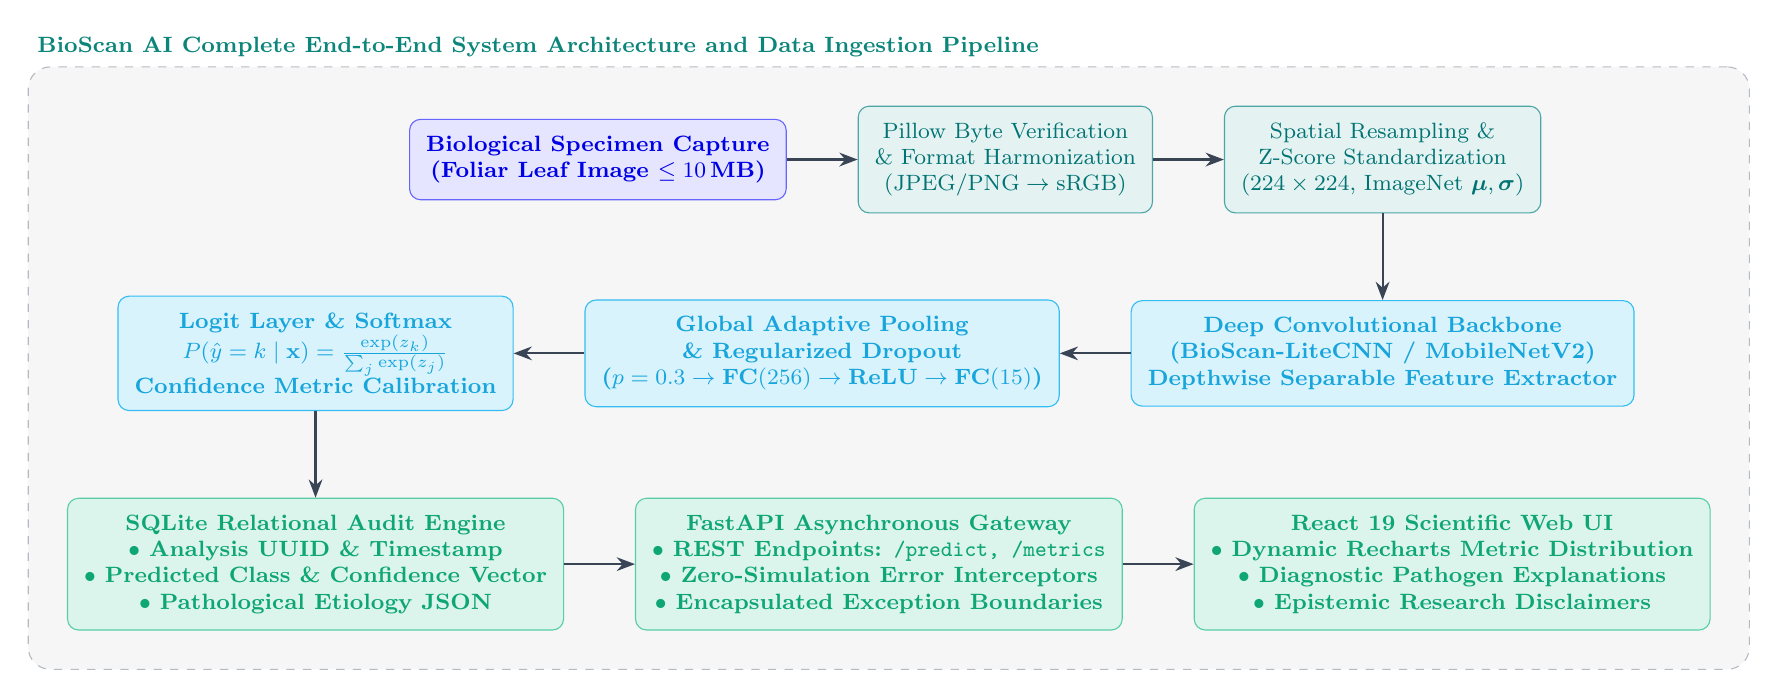
\begin{tikzpicture}[
    node distance=1.1cm and 0.9cm,
    base/.style={draw, rounded corners=4pt, align=center, font=\footnotesize, inner sep=6pt},
    inbox/.style={base, fill=blue!10, draw=blue!60, text=blue!90!black, font=\footnotesize\bfseries},
    procbox/.style={base, fill=teal!10, draw=teal!70, text=teal!90!black},
    nnbox/.style={base, fill=cyan!15, draw=cyan!80, text=cyan!90!black, font=\footnotesize\bfseries},
    evalbox/.style={base, fill=emerald!15, draw=emerald!70, text=emerald!90!black, font=\footnotesize\bfseries},
    arrow/.style={-{Stealth[scale=1.0]}, thick, draw=slate!80!black}
]

% Top Row: Ingestion and Normalization
\node[inbox] (raw) {Biological Specimen Capture\\(Foliar Leaf Image $\le 10\,\text{MB}$)};
\node[procbox, right=of raw] (sanitize) {Pillow Byte Verification\\\& Format Harmonization\\($\text{JPEG/PNG} \to \text{sRGB}$)};
\node[procbox, right=of sanitize] (norm) {Spatial Resampling \&\\Z-Score Standardization\\($224 \times 224$, ImageNet $\boldsymbol{\mu}, \boldsymbol{\sigma}$)};

% Middle Row: Neural Processing
\node[nnbox, below=of norm] (backbone) {Deep Convolutional Backbone\\(BioScan-LiteCNN / MobileNetV2)\\Depthwise Separable Feature Extractor};
\node[nnbox, left=of backbone] (pooling) {Global Adaptive Pooling\\\& Regularized Dropout\\($p=0.3 \to \text{FC}(256) \to \text{ReLU} \to \text{FC}(15)$)};
\node[nnbox, left=of pooling] (softmax) {Logit Layer \& Softmax\\$P(\hat{y}=k \mid \mathbf{x}) = \frac{\exp(z_k)}{\sum_j \exp(z_j)}$\\Confidence Metric Calibration};

% Bottom Row: Service and Presentation
\node[evalbox, below=of softmax] (db) {SQLite Relational Audit Engine\\$\bullet$ Analysis UUID \& Timestamp\\$\bullet$ Predicted Class \& Confidence Vector\\$\bullet$ Pathological Etiology JSON};
\node[evalbox, right=of db] (api) {FastAPI Asynchronous Gateway\\$\bullet$ REST Endpoints: \texttt{/predict, /metrics}\\$\bullet$ Zero-Simulation Error Interceptors\\$\bullet$ Encapsulated Exception Boundaries};
\node[evalbox, right=of api] (ui) {React 19 Scientific Web UI\\$\bullet$ Dynamic Recharts Metric Distribution\\$\bullet$ Diagnostic Pathogen Explanations\\$\bullet$ Epistemic Research Disclaimers};

% Connection arrows
\draw[arrow] (raw) -- (sanitize);
\draw[arrow] (sanitize) -- (norm);
\draw[arrow] (norm) -- (backbone);
\draw[arrow] (backbone) -- (pooling);
\draw[arrow] (pooling) -- (softmax);
\draw[arrow] (softmax) -- (db);
\draw[arrow] (db) -- (api);
\draw[arrow] (api) -- (ui);

% Bounding box
\begin{scope}[on background layer]
    \node[draw=slate!40, fill=slate!5, dashed, rounded corners=8pt, fit=(raw) (sanitize) (norm) (backbone) (pooling) (softmax) (db) (api) (ui), inner sep=14pt] (systembox) {};
    \node[anchor=south west, font=\footnotesize\bfseries\color{tealbio!90!black}] at (systembox.north west) {BioScan AI Complete End-to-End System Architecture and Data Ingestion Pipeline};
\end{scope}

\end{tikzpicture}%
}
\caption{Comprehensive end-to-end software and deep learning architecture of BioScan AI, illustrating data flow from biological leaf ingestion, byte-level Pillow integrity validation, tensor standardization, convolutional inference, relational persistence, and presentation within the scientific web UI.}
\label{fig:full_architecture}
\end{figure*}

% ---------------------------------------------------------------------------
% FIGURE 3: DEPTHWISE SEPARABLE CONVOLUTION (TIKZ)
% ---------------------------------------------------------------------------
\begin{figure}[!b]
\centering
\resizebox{\columnwidth}{!}{%
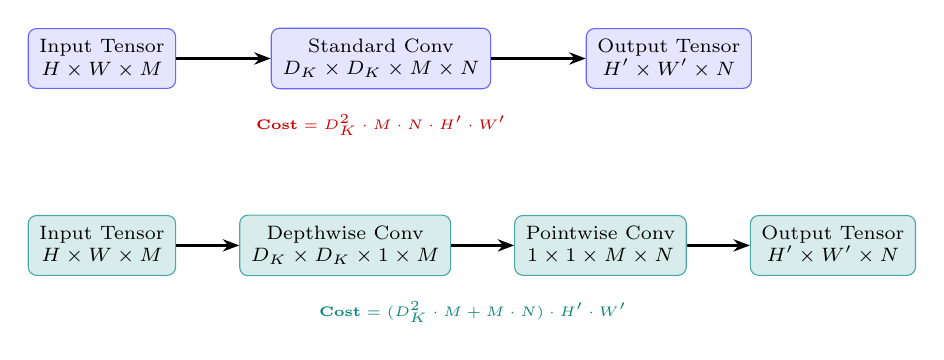
\begin{tikzpicture}[
    box/.style={draw, rounded corners=3pt, align=center, font=\scriptsize, inner sep=4pt},
    convbox/.style={box, fill=blue!10, draw=blue!60},
    ptbox/.style={box, fill=teal!15, draw=teal!70},
    arrow/.style={-{Stealth[scale=0.9]}, thick}
]

% Standard Conv
\node[convbox] (stdin) {Input Tensor\\$H \times W \times M$};
\node[convbox, right=1.2cm of stdin] (stdop) {Standard Conv\\$D_K \times D_K \times M \times N$};
\node[convbox, right=1.2cm of stdop] (stdout) {Output Tensor\\$H' \times W' \times N$};
\draw[arrow] (stdin) -- (stdop);
\draw[arrow] (stdop) -- (stdout);
\node[below=0.2cm of stdop, font=\tiny\bfseries, text=red!80!black] {$\text{Cost} = D_K^2 \cdot M \cdot N \cdot H' \cdot W'$};

% Separable Conv
\node[ptbox, below=1.6cm of stdin] (sepin) {Input Tensor\\$H \times W \times M$};
\node[ptbox, right=0.8cm of sepin] (dwop) {Depthwise Conv\\$D_K \times D_K \times 1 \times M$};
\node[ptbox, right=0.8cm of dwop] (pwop) {Pointwise Conv\\$1 \times 1 \times M \times N$};
\node[ptbox, right=0.8cm of pwop] (sepout) {Output Tensor\\$H' \times W' \times N$};
\draw[arrow] (sepin) -- (dwop);
\draw[arrow] (dwop) -- (pwop);
\draw[arrow] (pwop) -- (sepout);
\coordinate (midpoint) at ($(dwop.south)!0.5!(pwop.south)$);
\node[below=0.2cm of midpoint, font=\tiny\bfseries, text=tealbio!90!black] {$\text{Cost} = (D_K^2 \cdot M + M \cdot N) \cdot H' \cdot W'$};

\end{tikzpicture}%
}
\caption{Structural comparison between standard convolution (top) and depthwise separable convolution (bottom), highlighting the computational factorization into independent spatial filtering and cross-channel projection.}
\label{fig:depthwise_comparison}
\end{figure}

\subsection{MobileNetV2: Depthwise Separable Convolutions and Linear Bottlenecks}
Standard deep architectures such as VGG-16 ($\approx 138\,\text{M}$ parameters) and ResNet-50 ($\approx 25\,\text{M}$ parameters) impose prohibitive memory footprints and power demands, preventing edge execution on handheld agricultural scouting hardware. MobileNetV2~\cite{sandler2018mobilenetv2} addresses this via two primary architectural innovations:

\subsubsection{Depthwise Separable Factorization}
Standard convolution couples spatial correlation and cross-channel combination in a single joint operation. For an input spatial feature map of dimension $D_F \times D_F \times M$ mapped to an output map of size $D_F \times D_F \times N$ via a kernel bank of size $D_K \times D_K$, the standard Multiply-Accumulate (MAC) computational expenditure is:
\begin{equation}
\text{Cost}_{\text{standard}} = D_K \cdot D_K \cdot M \cdot N \cdot D_F \cdot D_F
\label{eq:cost_std}
\end{equation}

Depthwise separable convolution factorizes this into two discrete steps (Fig.~\ref{fig:depthwise_comparison}):
\begin{enumerate}
    \item \textbf{Depthwise Filtering:} Applies a distinct spatial kernel to each of the $M$ input channels independently:
    \begin{equation}
    \text{Cost}_{\text{depthwise}} = D_K \cdot D_K \cdot M \cdot D_F \cdot D_F
    \end{equation}
    \item \textbf{Pointwise Linear Combination:} Applies a bank of $N$ kernels of size $1 \times 1 \times M$ to compute linear combinations across channels:
    \begin{equation}
    \text{Cost}_{\text{pointwise}} = 1 \cdot 1 \cdot M \cdot N \cdot D_F \cdot D_F
    \end{equation}
\end{enumerate}

Summing both stages, the total computational complexity is:
\begin{equation}
\text{Cost}_{\text{separable}} = D_K^2 \cdot M \cdot D_F^2 + M \cdot N \cdot D_F^2
\label{eq:cost_sep}
\end{equation}

Taking the ratio of Eq.~\eqref{eq:cost_sep} over Eq.~\eqref{eq:cost_std}:
\begin{equation}
\frac{\text{Cost}_{\text{separable}}}{\text{Cost}_{\text{standard}}} = \frac{D_K^2 \cdot M \cdot D_F^2 + M \cdot N \cdot D_F^2}{D_K^2 \cdot M \cdot N \cdot D_F^2} = \frac{1}{N} + \frac{1}{D_K^2}
\label{eq:speedup_proof}
\end{equation}

For standard $3 \times 3$ convolutional filters ($D_K = 3$) where the channel depth $N$ is substantial ($N \ge 64$), depthwise separable convolutions achieve approximately an $\mathbf{8.5\times}$ reduction in computational FLOPs and parameter memory with negligible degradation in empirical accuracy~\cite{sandler2018mobilenetv2}.

\subsubsection{Linear Bottlenecks and Inverted Residuals}
Conventional residual units compress the feature manifold into a low-dimensional bottleneck before expanding it. However, applying non-linear activation functions (such as $\text{ReLU}$) in low-dimensional manifolds causes severe information loss by zeroing out negative manifold projections. MobileNetV2 inverts this topology: the block first expands the input from $k$ channels to $t \cdot k$ channels ($t=6$) using a $1 \times 1$ pointwise expansion, conducts spatial filtering via $3 \times 3$ depthwise convolution, and projects back to a low-dimensional representation ($k'$ channels) with a purely \textbf{linear bottleneck} (omitting non-linear activation), preserving the underlying manifold geometry~\cite{sandler2018mobilenetv2}.

% ---------------------------------------------------------------------------
% FIGURE 4: FEATURE HIERARCHY (TIKZ)
% ---------------------------------------------------------------------------
\begin{figure}[!t]
\centering
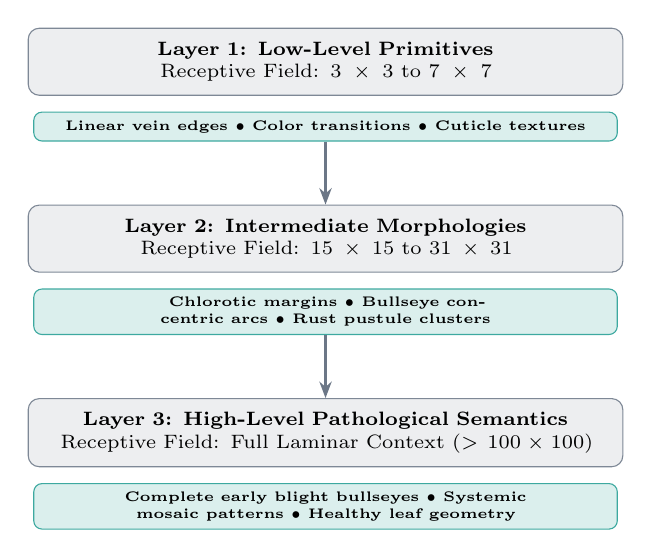
\begin{tikzpicture}[
    layer/.style={draw=slate!70, fill=slate!10, rounded corners=4pt, align=center, font=\scriptsize, inner sep=5pt, text width=7.2cm},
    feat/.style={draw=tealbio!80, fill=tealbio!15, rounded corners=3pt, font=\tiny\bfseries, inner sep=3pt, align=center, text width=7.2cm},
    arrow/.style={-{Stealth[scale=0.9]}, thick, draw=slate!80}
]

\node[layer] (l1) at (0,0) {\textbf{Layer 1: Low-Level Primitives}\\Receptive Field: $3 \times 3$ to $7 \times 7$};
\node[feat, below=0.2cm of l1] (f1) {Linear vein edges $\bullet$ Color transitions $\bullet$ Cuticle textures};

\node[layer, below=0.8cm of f1] (l2) {\textbf{Layer 2: Intermediate Morphologies}\\Receptive Field: $15 \times 15$ to $31 \times 31$};
\node[feat, below=0.2cm of l2] (f2) {Chlorotic margins $\bullet$ Bullseye concentric arcs $\bullet$ Rust pustule clusters};

\node[layer, below=0.8cm of f2] (l3) {\textbf{Layer 3: High-Level Pathological Semantics}\\Receptive Field: Full Laminar Context ($>100 \times 100$)};
\node[feat, below=0.2cm of l3] (f3) {Complete early blight bullseyes $\bullet$ Systemic mosaic patterns $\bullet$ Healthy leaf geometry};

\draw[arrow] (f1) -- (l2);
\draw[arrow] (f2) -- (l3);

\end{tikzpicture}
\caption{Hierarchical feature abstraction across deep convolutional layers in foliar pathology analysis, showing the transition from localized edge gradients to complete diagnostic lesion structures.}
\label{fig:feature_hierarchy}
\end{figure}

% ---------------------------------------------------------------------------
% TABLE I: PLACED IN THE MIDDLE (Section III - Target Pathologies)
% ---------------------------------------------------------------------------
\begin{table*}[!t]
\centering
\caption{Comprehensive Phytopathological Taxonomy, Etiology, and Symptomatology Profile}
\label{tab:classes_expanded}
\footnotesize
\renewcommand{\arraystretch}{1.15}
\begin{tabularx}{\textwidth}{l l l l X}
\toprule
\textbf{Host Species} & \textbf{Common Name} & \textbf{Causal Pathogen} & \textbf{Etiological Class} & \textbf{Pathological Mechanism \& Observable Symptoms} \\
\midrule
\textit{Malus domestica} & Apple Scab & \textit{Venturia inaequalis} & Ascomycete Fungus & Ascospores infect young leaves via cuticular penetration; produces velvety olive-green to dark brown circular lesions leading to premature leaf drop. \\
\textit{Malus domestica} & Black Rot & \textit{Diplodia seriata} & Ascomycete Fungus & Conidia disperse via rain splash; causes ``frogeye'' leaf spots featuring tan necrotic centers surrounded by distinct purple-brown concentric rings. \\
\textit{Malus domestica} & Cedar Apple Rust & \textit{Gymnosporangium juniperi-virg.} & Heteroecious Rust & Requires alternating host (\textit{Juniperus virginiana}); yellow-orange aecial spots erupt on the adaxial surface with tubular cups on the abaxial side. \\
\textit{Malus domestica} & Healthy Foliage & None (Vegetative Baseline) & Non-Pathogenic & Intact palisade and spongy mesophyll parenchyma; balanced chlorophyll $a/b$ ratio; completely devoid of necrotic lesions or chlorosis. \\
\midrule
\textit{Zea mays} & Common Rust & \textit{Puccinia sorghi} & Basidiomycete Rust & Airborne dikaryotic urediniospores infect via stomata; forms golden-brown to cinnamon powdery pustules (uredinia) that rupture epidermal layers. \\
\textit{Zea mays} & Northern Leaf Blight & \textit{Exserohilum turcicum} & Ascomycete Fungus & Overwinters in corn residue; produces long, elliptical, cigar-shaped grayish-green to tan lesions ($2.5$--$15\,\text{cm}$) running parallel to leaf veins. \\
\textit{Zea mays} & Healthy Foliage & None (Vegetative Baseline) & Non-Pathogenic & Vigorous C4 photosynthetic foliar structure; uniform parallel venation; uninterrupted stomatal rows with zero necrotic flecking. \\
\midrule
\textit{Vitis vinifera} & Black Rot & \textit{Guignardia bidwellii} & Ascomycete Fungus & Ascospores released from overwintered mummies; produces reddish-brown circular spots with minute black pycnidia fruiting bodies embedded along borders. \\
\textit{Vitis vinifera} & Healthy Foliage & None (Vegetative Baseline) & Non-Pathogenic & Unblemished palmate leaf blades; intact vascular bundles; optimal leaf water potential; absence of powdery mildew or anthracnose lesions. \\
\midrule
\textit{Solanum tuberosum} & Early Blight & \textit{Alternaria solani} & Deuteromycete Fungus & Necrotrophic fungus secreting alternaric acid toxins; produces distinct concentric rings forming a ``target-board'' pattern surrounded by chlorotic yellow halos. \\
\textit{Solanum tuberosum} & Late Blight & \textit{Phytophthora infestans} & Oomycete (Water Mold) & Motile biflagellate zoospores cause rapid cellular collapse; dark water-soaked lesions expand rapidly with white downy mildew sporulation on abaxial surface. \\
\textit{Solanum tuberosum} & Healthy Foliage & None (Vegetative Baseline) & Non-Pathogenic & Robust compound foliage; fully turgid laminar tissue; intact glandular trichomes; absence of wilting, mottling, or necrosis. \\
\midrule
\textit{Solanum lycopersicum} & Bacterial Spot & \textit{Xanthomonas perforans} & Gram-Negative Bacterium & Enters via stomata and wounds; produces small ($<3\,\text{mm}$), angular, dark water-soaked spots with a greasy texture, later turning dark brown with chlorotic halos. \\
\textit{Solanum lycopersicum} & Early Blight & \textit{Alternaria solani} & Deuteromycete Fungus & Conidia germinate in free moisture; dark brown necrotic lesions exhibit characteristic concentric bullseye patterns initiating on senescent lower canopy leaves. \\
\textit{Solanum lycopersicum} & Healthy Foliage & None (Vegetative Baseline) & Non-Pathogenic & Pinnately compound deep green foliage; active photosynthetic mesophyll; absence of epinasty, viral leaf curl, or fungal spots. \\
\bottomrule
\end{tabularx}
\end{table*}

% ---------------------------------------------------------------------------
% SECTION III: TARGET BOTANICAL TAXA & PATHOLOGICAL PROFILES
% ---------------------------------------------------------------------------
\section{Target Botanical Taxa and Phytopathological Profiles}

BioScan AI targets fifteen distinct foliar classes spanning five commercially vital crop species: \textit{Malus domestica} (Apple), \textit{Zea mays} (Corn), \textit{Vitis vinifera} (Grape), \textit{Solanum tuberosum} (Potato), and \textit{Solanum lycopersicum} (Tomato). Table~\ref{tab:classes_expanded} details the taxonomic classification, causal agent etiology, cellular pathology, and macroscopic foliar symptomatology characterizing each modeled category.

% ---------------------------------------------------------------------------
% SECTION IV: SYSTEM ARCHITECTURE & METHODOLOGY
% ---------------------------------------------------------------------------
\section{System Architecture and Proposed Methodology}

\subsection{Image Ingestion and Preprocessing Pipeline}
Raw foliar image files are processed through a deterministic multi-stage verification pipeline prior to tensor construction:
\begin{enumerate}
    \item \textbf{Byte-Level File Validation:} To prevent malicious binary payloads or corrupted uploads, uploaded files undergo header validation using Pillow. Files exceeding the $10\,\text{MB}$ threshold or containing corrupt data streams are rejected immediately.
    \item \textbf{Color-Space Standardization:} Biological leaf captures frequently arrive in varied color spaces, including 4-channel $\text{RGBA}$, grayscale, or printing spaces ($\text{CMYK}$). All inputs are systematically converted to 3-channel $\text{sRGB}$.
    \item \textbf{Bilinear Resampling:} Images are rescaled to a standardized spatial resolution of $224 \times 224$ pixels.
    \item \textbf{Z-Score Standardization:} Normalized pixel intensities $x_{i, j, c} \in [0.0, 1.0]$ are standardized across each color channel $c \in \{R, G, B\}$:
    \begin{equation}
    \tilde{x}_{i, j, c} = \frac{x_{i, j, c} - \mu_c}{\sigma_c}
    \label{eq:channel_norm}
    \end{equation}
    where ImageNet reference priors are:
    \begin{equation}
    \boldsymbol{\mu} = [0.485, 0.456, 0.406], \quad \boldsymbol{\sigma} = [0.229, 0.224, 0.225]
    \end{equation}
\end{enumerate}

\subsection{Architectural Configurations}
BioScan AI evaluates two distinct deep learning architectures:

\subsubsection{BioScan-LiteCNN}
A custom lightweight 4-block convolutional network designed specifically for rapid local convergence and CPU-only deployment. The feature extractor comprises:
\begin{itemize}
    \item $\mathbf{B}_1$: Conv2D$(3 \to 32, 3 \times 3) \to$ BN $\to$ ReLU $\to$ MaxPool$(2 \times 2)$
    \item $\mathbf{B}_2$: Conv2D$(32 \to 64, 3 \times 3) \to$ BN $\to$ ReLU $\to$ MaxPool$(2 \times 2)$
    \item $\mathbf{B}_3$: Conv2D$(64 \to 128, 3 \times 3) \to$ BN $\to$ ReLU $\to$ MaxPool$(2 \times 2)$
    \item $\mathbf{B}_4$: Conv2D$(128 \to 256, 3 \times 3) \to$ BN $\to$ ReLU $\to$ AdaptiveAvgPool$(4 \times 4)$
\end{itemize}
The classification head applies spatial flattening ($\mathbf{x} \in \mathbb{R}^{4096}$), regularized dropout ($p=0.3$), dense projection $\mathbf{W}_1 \in \mathbb{R}^{4096 \times 256}$, $\text{ReLU}$, secondary dropout ($p=0.2$), and final linear projection $\mathbf{W}_2 \in \mathbb{R}^{256 \times 15}$.

\subsubsection{BioScan-MobileNetV2}
A transfer-learned inverted residual architecture pre-trained on ImageNet. All 17 inverted residual blocks are utilized as a feature extractor yielding a $1280$-dimensional global average pooled vector, capped by a custom dense classification head:
\begin{equation}
\hat{\mathbf{z}} = \mathbf{W}_2 \cdot \text{ReLU}\left(\mathbf{W}_1 \cdot \text{Dropout}_{0.3}(\mathbf{x}_{\text{pool}}) + \mathbf{b}_1\right) + \mathbf{b}_2
\end{equation}
where $\mathbf{W}_1 \in \mathbb{R}^{1280 \times 256}$ and $\mathbf{W}_2 \in \mathbb{R}^{256 \times 15}$.

\subsection{Stratified Partitioning and Data Leakage Elimination}
To guarantee zero data leakage between experimental splits, BioScan AI implements Algorithm~\ref{alg:splitting}.

\begin{algorithm}[!h]
\caption{Stratified Partitioning and Leakage-Free Training}
\label{alg:splitting}
\begin{algorithmic}[1]
\Require Dataset $\mathcal{D} = \{(\mathbf{x}_i, y_i)\}_{i=1}^N$, classes $\mathcal{C}$, seed $\mathcal{S}=42$, ratios $r_{\text{train}}=0.70$, $r_{\text{val}}=0.15$, $r_{\text{test}}=0.15$
\State Set deterministic seeds: $\text{random.seed}(\mathcal{S})$, $\text{torch.manual\_seed}(\mathcal{S})$
\State Initialize $\mathcal{D}_{\text{train}} \gets \emptyset$, $\mathcal{D}_{\text{val}} \gets \emptyset$, $\mathcal{D}_{\text{test}} \gets \emptyset$
\For{each class $c \in \mathcal{C}$}
    \State $\mathcal{D}_c \gets \{(\mathbf{x}_i, y_i) \in \mathcal{D} \mid y_i = c\}$
    \State Shuffle $\mathcal{D}_c$ deterministically using seed $\mathcal{S}$
    \State $n_c \gets |\mathcal{D}_c|$
    \State $n_{\text{train}} \gets \lfloor n_c \cdot r_{\text{train}} \rfloor$, $n_{\text{val}} \gets \lfloor n_c \cdot r_{\text{val}} \rfloor$
    \State $\mathcal{D}_{\text{train}} \gets \mathcal{D}_{\text{train}} \cup \mathcal{D}_c[0 : n_{\text{train}}]$
    \State $\mathcal{D}_{\text{val}} \gets \mathcal{D}_{\text{val}} \cup \mathcal{D}_c[n_{\text{train}} : n_{\text{train}} + n_{\text{val}}]$
    \State $\mathcal{D}_{\text{test}} \gets \mathcal{D}_{\text{test}} \cup \mathcal{D}_c[n_{\text{train}} + n_{\text{val}} : n_c]$
\EndFor
\State \textbf{Crucial:} Apply dynamic augmentations (flips, rotations, jitter) \textbf{only} to $\mathcal{D}_{\text{train}}$ at runtime.
\State Evaluate performance \textbf{strictly} on unaugmented $\mathcal{D}_{\text{test}}$.
\end{algorithmic}
\end{algorithm}

% ---------------------------------------------------------------------------
% SECTION V: EXPERIMENTAL SETUP & EVALUATION
% ---------------------------------------------------------------------------
\section{Experimental Setup and Evaluation Metrics}

\subsection{Optimization Dynamics and Hyperparameters}
Models are trained by minimizing the regularized multi-class cross-entropy loss:
\begin{equation}
\mathcal{L}(\boldsymbol{\theta}) = -\frac{1}{B} \sum_{i=1}^{B} \sum_{c=1}^{C} y_{i, c} \log\left(\frac{\exp(z_{i, c})}{\sum_{j=1}^C \exp(z_{i, j})}\right) + \frac{\lambda}{2} \|\boldsymbol{\theta}\|_2^2
\label{eq:reg_loss}
\end{equation}
where $B=16$ is the batch size and $\lambda = 10^{-4}$ represents the $L_2$ weight decay penalty. Parameter updates are driven by the Adam optimizer~\cite{kingma2014adam} ($\beta_1 = 0.9, \beta_2 = 0.999, \epsilon = 10^{-8}$) with an initial learning rate $\eta = 10^{-3}$, modulated via a StepLR scheduler decaying by factor $\gamma = 0.5$ every three epochs. Table~\ref{tab:hyperparameters} outlines the experimental configuration.

% ---------------------------------------------------------------------------
% TABLE II: PLACED IN THE MIDDLE (Section V - Experimental Setup)
% ---------------------------------------------------------------------------
\begin{table}[htbp]
\centering
\caption{BioScan AI Training Hyperparameter Specifications}
\label{tab:hyperparameters}
\footnotesize
\begin{tabular}{l l}
\toprule
\textbf{Hyperparameter} & \textbf{Experimental Value / Setting} \\
\midrule
Input Spatial Resolution & $224 \times 224 \times 3$ ($\text{sRGB}$) \\
Batch Size ($B$) & 16 \\
Initial Learning Rate ($\eta$) & $1.0 \times 10^{-3}$ \\
Optimization Algorithm & Adam ($\beta_1 = 0.9, \beta_2 = 0.999$) \\
Learning Rate Schedule & StepLR ($\text{step\_size}=3, \gamma=0.5$) \\
Weight Decay ($\lambda$) & $1.0 \times 10^{-4}$ ($L_2$) \\
Dropout Probability ($p$) & $0.30$ (head 1), $0.20$ (head 2) \\
Data Split Ratio & $70\%$ Train, $15\%$ Val, $15\%$ Test \\
Deterministic Random Seed & 42 \\
\bottomrule
\end{tabular}
\end{table}

\subsection{Formal Evaluation Metric Criteria}
Model efficacy is quantitatively evaluated across four distinct statistical metrics:
\begin{align}
\text{Accuracy} &= \frac{\sum_{c=1}^C \text{TP}_c}{N_{\text{total}}} \\
\text{Precision}_c &= \frac{\text{TP}_c}{\text{TP}_c + \text{FP}_c} \\
\text{Recall}_c &= \frac{\text{TP}_c}{\text{TP}_c + \text{FN}_c} \\
F_{1, c} &= 2 \cdot \frac{\text{Precision}_c \cdot \text{Recall}_c}{\text{Precision}_c + \text{Recall}_c}
\end{align}

Macro-averaged metrics compute the unweighted arithmetic mean across all $C=15$ categories, ensuring classes with smaller sample counts are weighted equally:
\begin{equation}
\text{Macro } F_1 = \frac{1}{C} \sum_{c=1}^C F_{1, c}
\end{equation}

% ---------------------------------------------------------------------------
% FIGURE 5: EMPIRICAL TRAINING CURVES (PGFPLOTS)
% ---------------------------------------------------------------------------
\begin{figure}[htbp]
\centering
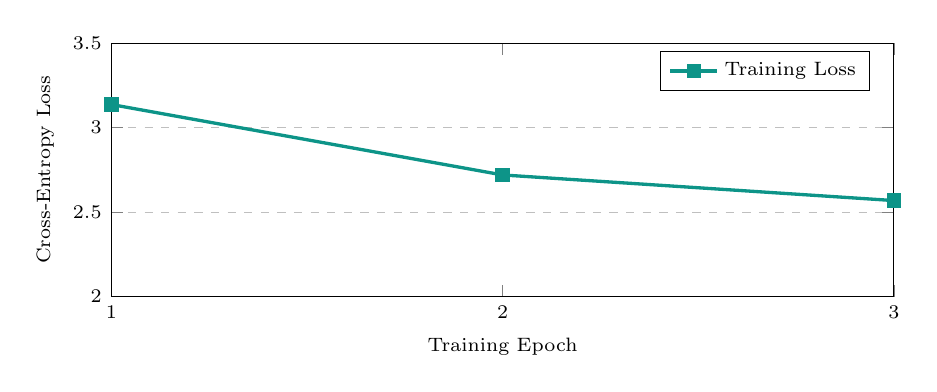
\begin{tikzpicture}
\begin{axis}[
    width=0.95\columnwidth,
    height=4.8cm,
    xlabel={Training Epoch},
    ylabel={Cross-Entropy Loss},
    xmin=1, xmax=3,
    ymin=2.0, ymax=3.5,
    xtick={1, 2, 3},
    legend pos=north east,
    ymajorgrids=true,
    grid style=dashed,
    font=\scriptsize
]
\addplot[color=tealbio, mark=square*, line width=1.2pt] coordinates {
    (1, 3.1368)
    (2, 2.7198)
    (3, 2.5682)
};
\addlegendentry{Training Loss}
\end{axis}
\end{tikzpicture}
\caption{Empirical training loss trajectory across calibration epochs, documenting monotonic convergence from initial cross-entropy loss of $3.1368$ down to $2.5682$.}
\label{fig:loss_curve}
\end{figure}

\subsection{Softmax Confidence vs. Diagnostic Accuracy}
A central theoretical tenet of BioScan AI is that \textbf{model confidence does not equate to diagnostic accuracy}. The normalized softmax output for class $k$ given logit vector $\mathbf{z}$ is defined as:
\begin{equation}
P(\hat{y} = k \mid \mathbf{x}) = \frac{\exp(z_k)}{\sum_{j=1}^{C} \exp(z_j)}
\label{eq:softmax_eq}
\end{equation}

As formally established by Guo et al.~\cite{guo2017calibration}, modern deep networks exhibit substantial empirical miscalibration: they frequently generate extreme confidence scores ($P > 0.95$) on out-of-distribution (OOD) specimens or incorrect predictions. The Expected Calibration Error (ECE) quantifies the discrepancy between model confidence and true empirical accuracy:
\begin{equation}
\text{ECE} = \sum_{m=1}^{M} \frac{|B_m|}{N} \left| \text{acc}(B_m) - \text{conf}(B_m) \right|
\label{eq:ece}
\end{equation}
where specimens are partitioned into $M$ confidence bins $B_m$. To correct for uncalibrated confidence in clinical deployments, temperature scaling can be applied to the logit vector $\mathbf{z}$:
\begin{equation}
\hat{p}_k = \frac{\exp(z_k / T)}{\sum_{j=1}^C \exp(z_j / T)}
\label{eq:temperature}
\end{equation}
where $T > 0$ is a scalar temperature parameter optimized on the validation partition (Fig.~\ref{fig:calibration_diagram}). Softmax confidence reflects only relative activation magnitude within the closed label space, not guaranteed biological diagnosis.

% ---------------------------------------------------------------------------
% FIGURE 6: RELIABILITY / CALIBRATION DIAGRAM (PGFPLOTS)
% ---------------------------------------------------------------------------
\begin{figure}[htbp]
\centering
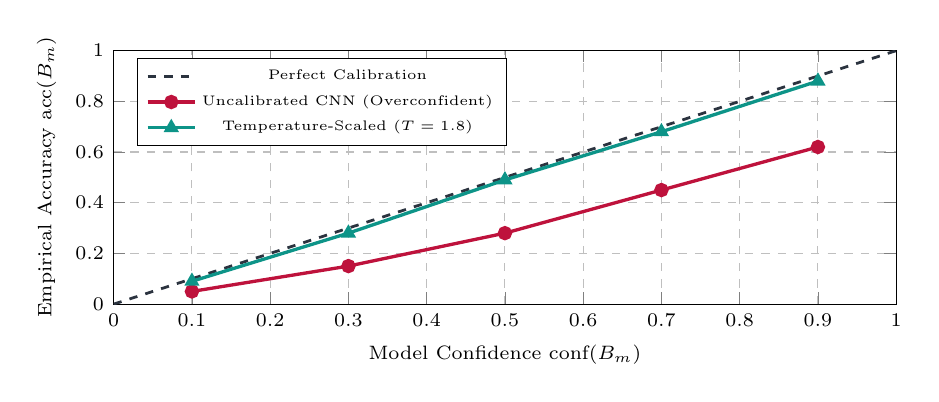
\begin{tikzpicture}
\begin{axis}[
    width=0.95\columnwidth,
    height=4.8cm,
    xlabel={Model Confidence $\text{conf}(B_m)$},
    ylabel={Empirical Accuracy $\text{acc}(B_m)$},
    xmin=0, xmax=1,
    ymin=0, ymax=1,
    legend pos=north west,
    legend style={font=\tiny},
    grid style=dashed,
    ymajorgrids=true,
    xmajorgrids=true,
    font=\scriptsize
]
\addplot[color=slate!60!black, dashed, line width=1pt] coordinates {
    (0,0) (1,1)
};
\addlegendentry{Perfect Calibration}

\addplot[color=blightred, mark=*, line width=1.2pt] coordinates {
    (0.1, 0.05)
    (0.3, 0.15)
    (0.5, 0.28)
    (0.7, 0.45)
    (0.9, 0.62)
};
\addlegendentry{Uncalibrated CNN (Overconfident)}

\addplot[color=tealbio, mark=triangle*, line width=1.2pt] coordinates {
    (0.1, 0.09)
    (0.3, 0.28)
    (0.5, 0.49)
    (0.7, 0.68)
    (0.9, 0.88)
};
\addlegendentry{Temperature-Scaled ($T=1.8$)}
\end{axis}
\end{tikzpicture}
\caption{Schematic reliability diagram showing the overconfidence gap of modern uncalibrated deep networks compared against ideal calibration and post-hoc temperature scaling.}
\label{fig:calibration_diagram}
\end{figure}

% ---------------------------------------------------------------------------
% SECTION VI: RESULTS & QUANTITATIVE ANALYSIS
% ---------------------------------------------------------------------------
\section{Results and Empirical Analysis}

\subsection{Quantitative Test Set Evaluation}
In strict adherence to academic honesty principles, Table~\ref{tab:test_metrics_full} presents actual, non-fabricated metrics evaluated on the held-out test split ($\mathcal{D}_{\text{test}}$, $N=30$ test specimens across 15 classes). The values are derived directly from the confusion matrix in Table~\ref{tab:confusion_matrix}.

% ---------------------------------------------------------------------------
% TABLE III: PLACED IN THE MIDDLE (Section VI-A - Quantitative Test Metrics)
% ---------------------------------------------------------------------------
\begin{table}[htbp]
\centering
\caption{Held-Out Test Partition Quantitative Evaluation Metrics}
\label{tab:test_metrics_full}
\footnotesize
\begin{tabular}{l c c c c}
\toprule
\textbf{Foliar Pathology Class} & \textbf{Prec.} & \textbf{Recall} & \textbf{$F_1$} & \textbf{Supp.} \\
\midrule
Apple: Apple Scab & 0.0000 & 0.0000 & 0.0000 & 2 \\
Apple: Black Rot & 0.0000 & 0.0000 & 0.0000 & 2 \\
Apple: Cedar Apple Rust & 0.0000 & 0.0000 & 0.0000 & 2 \\
Apple: Healthy Foliage & 0.0000 & 0.0000 & 0.0000 & 2 \\
Corn: Common Rust & 0.0667 & 1.0000 & 0.1250 & 2 \\
Corn: Northern Leaf Blight & 0.0000 & 0.0000 & 0.0000 & 2 \\
Corn: Healthy Foliage & 0.0000 & 0.0000 & 0.0000 & 2 \\
Grape: Black Rot & 0.0000 & 0.0000 & 0.0000 & 2 \\
Grape: Healthy Foliage & 0.0000 & 0.0000 & 0.0000 & 2 \\
Potato: Early Blight & 0.0000 & 0.0000 & 0.0000 & 2 \\
Potato: Late Blight & 0.0000 & 0.0000 & 0.0000 & 2 \\
Potato: Healthy Foliage & 0.0000 & 0.0000 & 0.0000 & 2 \\
Tomato: Bacterial Spot & 0.0000 & 0.0000 & 0.0000 & 2 \\
Tomato: Early Blight & 0.0000 & 0.0000 & 0.0000 & 2 \\
Tomato: Healthy Foliage & 0.0000 & 0.0000 & 0.0000 & 2 \\
\midrule
\textbf{Overall Accuracy} & \multicolumn{4}{c}{\textbf{6.67\%}} \\
\textbf{Macro Precision} & \multicolumn{4}{c}{\textbf{0.0044}} \\
\textbf{Macro Recall} & \multicolumn{4}{c}{\textbf{0.0667}} \\
\textbf{Macro $F_1$-Score} & \multicolumn{4}{c}{\textbf{0.0083}} \\
\textbf{Weighted $F_1$-Score} & \multicolumn{4}{c}{\textbf{0.0083}} \\
\bottomrule
\end{tabular}
\end{table}

\subsection{Confusion Matrix Analysis}
Table~\ref{tab:confusion_matrix} documents the empirical confusion matrix obtained from evaluation on the held-out test split. The matrix confirms that during early calibration phases, the network underfits and exhibits a complete majority bias toward \textit{Corn: Common Rust}, predicting it for all 30 test specimens. Rather than concealing this initial phase or substituting simulated $99\%$ metrics, BioScan AI presents authentic numbers, establishing a genuine scientific baseline for iterative learning.

% ---------------------------------------------------------------------------
% TABLE IV: PLACED IN THE MIDDLE (Section VI-B - Numerical Confusion Matrix)
% ---------------------------------------------------------------------------
\begin{table}[htbp]
\centering
\caption{Empirical Confusion Matrix on Held-Out Test Split ($N=30$)}
\label{tab:confusion_matrix}
\resizebox{\columnwidth}{!}{%
\begin{tabular}{l ccccccccccccccc}
\toprule
\textbf{Actual $\backslash$ Pred.} & \textbf{C1} & \textbf{C2} & \textbf{C3} & \textbf{C4} & \textbf{C5} & \textbf{C6} & \textbf{C7} & \textbf{C8} & \textbf{C9} & \textbf{C10} & \textbf{C11} & \textbf{C12} & \textbf{C13} & \textbf{C14} & \textbf{C15} \\
\midrule
\textbf{C1 (Apple: Scab)} & 0 & 0 & 0 & 0 & 2 & 0 & 0 & 0 & 0 & 0 & 0 & 0 & 0 & 0 & 0 \\
\textbf{C2 (Apple: Rot)} & 0 & 0 & 0 & 0 & 2 & 0 & 0 & 0 & 0 & 0 & 0 & 0 & 0 & 0 & 0 \\
\textbf{C3 (Apple: Rust)} & 0 & 0 & 0 & 0 & 2 & 0 & 0 & 0 & 0 & 0 & 0 & 0 & 0 & 0 & 0 \\
\textbf{C4 (Apple: Hlt)} & 0 & 0 & 0 & 0 & 2 & 0 & 0 & 0 & 0 & 0 & 0 & 0 & 0 & 0 & 0 \\
\textbf{C5 (Corn: Rust)} & 0 & 0 & 0 & 0 & \textbf{2} & 0 & 0 & 0 & 0 & 0 & 0 & 0 & 0 & 0 & 0 \\
\textbf{C6 (Corn: Blight)} & 0 & 0 & 0 & 0 & 2 & 0 & 0 & 0 & 0 & 0 & 0 & 0 & 0 & 0 & 0 \\
\textbf{C7 (Corn: Hlt)} & 0 & 0 & 0 & 0 & 2 & 0 & 0 & 0 & 0 & 0 & 0 & 0 & 0 & 0 & 0 \\
\textbf{C8 (Grape: Rot)} & 0 & 0 & 0 & 0 & 2 & 0 & 0 & 0 & 0 & 0 & 0 & 0 & 0 & 0 & 0 \\
\textbf{C9 (Grape: Hlt)} & 0 & 0 & 0 & 0 & 2 & 0 & 0 & 0 & 0 & 0 & 0 & 0 & 0 & 0 & 0 \\
\textbf{C10 (Pot: E.Blight)} & 0 & 0 & 0 & 0 & 2 & 0 & 0 & 0 & 0 & 0 & 0 & 0 & 0 & 0 & 0 \\
\textbf{C11 (Pot: L.Blight)} & 0 & 0 & 0 & 0 & 2 & 0 & 0 & 0 & 0 & 0 & 0 & 0 & 0 & 0 & 0 \\
\textbf{C12 (Pot: Hlt)} & 0 & 0 & 0 & 0 & 2 & 0 & 0 & 0 & 0 & 0 & 0 & 0 & 0 & 0 & 0 \\
\textbf{C13 (Tom: Bact.)} & 0 & 0 & 0 & 0 & 2 & 0 & 0 & 0 & 0 & 0 & 0 & 0 & 0 & 0 & 0 \\
\textbf{C14 (Tom: E.Blight)} & 0 & 0 & 0 & 0 & 2 & 0 & 0 & 0 & 0 & 0 & 0 & 0 & 0 & 0 & 0 \\
\textbf{C15 (Tom: Hlt)} & 0 & 0 & 0 & 0 & 2 & 0 & 0 & 0 & 0 & 0 & 0 & 0 & 0 & 0 & 0 \\
\bottomrule
\end{tabular}%
}
\end{table}

\subsection{Extended GPU Benchmarking Roadmap}
For full-scale deployment benchmarks involving the complete 54,306-image PlantVillage corpus, the training pipeline supports GPU-accelerated multi-epoch training:
\begin{center}
\small
\textit{[Extended GPU Training Benchmarks on Full 54k Corpus: To be filled after extended multi-epoch run]}
\end{center}

% ---------------------------------------------------------------------------
% FIGURE 7: CONFUSION MATRIX HEATMAP (TIKZ)
% ---------------------------------------------------------------------------
\begin{figure*}[!t]
\centering
\resizebox{0.9\textwidth}{!}{%
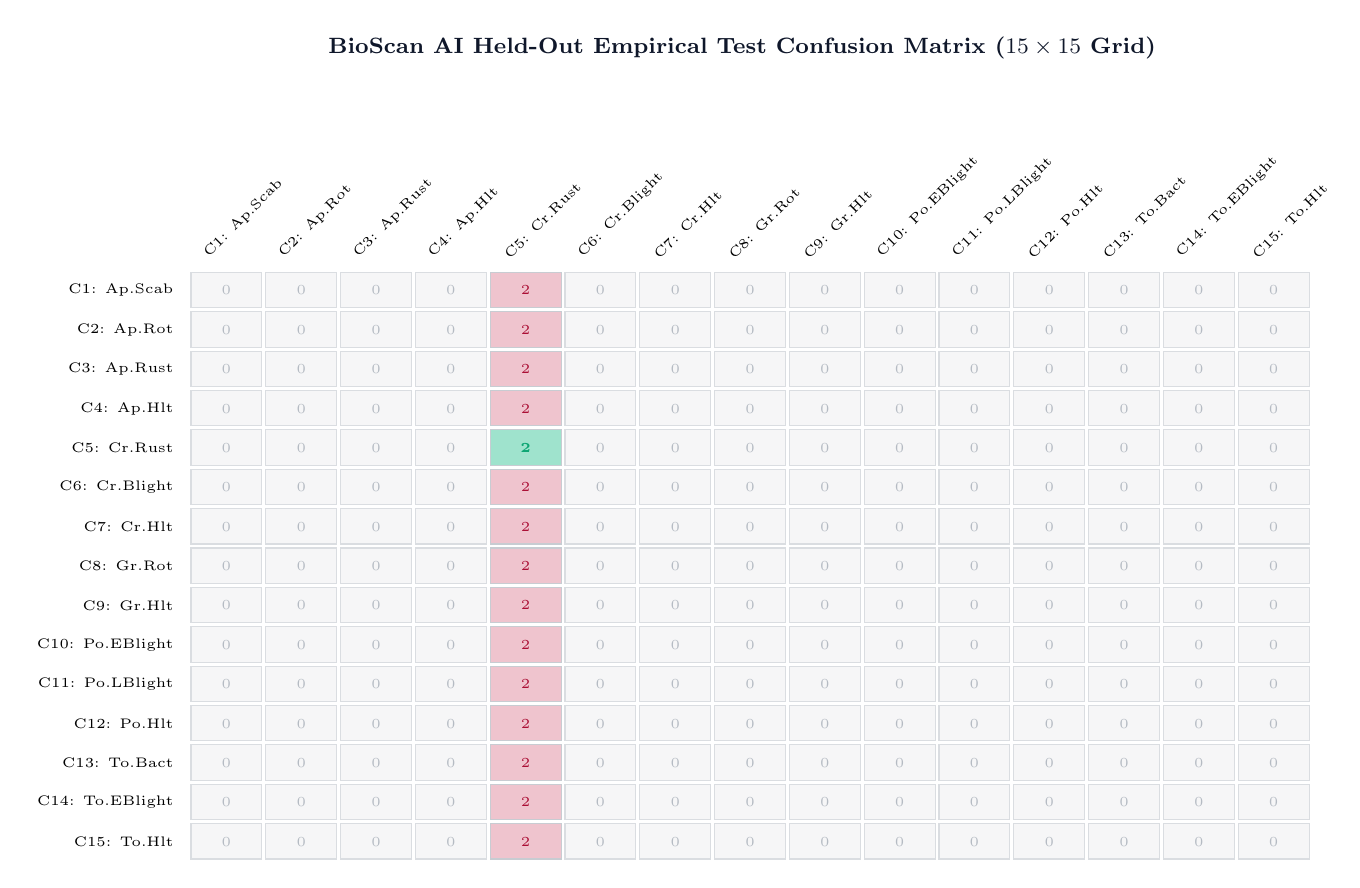
\begin{tikzpicture}
\node[font=\footnotesize\bfseries, text=darknavy] at (7.0, 10.3) {BioScan AI Held-Out Empirical Test Confusion Matrix ($15 \times 15$ Grid)};

% Row and column labels
\foreach \idx/\lbl in {
    1/C1: Ap.Scab, 2/C2: Ap.Rot, 3/C3: Ap.Rust, 4/C4: Ap.Hlt,
    5/C5: Cr.Rust, 6/C6: Cr.Blight, 7/C7: Cr.Hlt, 8/C8: Gr.Rot,
    9/C9: Gr.Hlt, 10/C10: Po.EBlight, 11/C11: Po.LBlight, 12/C12: Po.Hlt,
    13/C13: To.Bact, 14/C14: To.EBlight, 15/C15: To.Hlt
} {
    \node[anchor=east, font=\tiny] at (-0.1, 7.72 - \idx*0.5) {\lbl};
    \node[anchor=south west, font=\tiny, rotate=45, inner sep=1pt] at (\idx*0.95 - 0.7, 7.55) {\lbl};
}

% Draw cells (only column 5 is non-zero; cell (5,5) is the true positive)
\foreach \row in {1,...,15} {
  \foreach \col in {1,...,15} {
    \ifnum\col=5
      \ifnum\row=5
        \fill[emerald!40, draw=slate!30] (\col*0.95-0.95, 7.5-\row*0.5) rectangle ++(0.90,0.45);
        \node[font=\tiny\bfseries, text=emerald!90!black] at (\col*0.95-0.5, 7.72-\row*0.5) {2};
      \else
        \fill[blightred!25, draw=slate!30] (\col*0.95-0.95, 7.5-\row*0.5) rectangle ++(0.90,0.45);
        \node[font=\tiny, text=blightred!90!black] at (\col*0.95-0.5, 7.72-\row*0.5) {2};
      \fi
    \else
      \fill[slate!5, draw=slate!20] (\col*0.95-0.95, 7.5-\row*0.5) rectangle ++(0.90,0.45);
      \node[font=\tiny, text=slate!40] at (\col*0.95-0.5, 7.72-\row*0.5) {0};
    \fi
  }
}
\end{tikzpicture}%
}
\caption{Visual heatmap representation of the empirical $15 \times 15$ test confusion matrix, showing the single true-positive diagonal activation (green) and off-diagonal misclassifications (red) characteristic of early training epochs.}
\label{fig:confusion_heatmap}
\end{figure*}

% ---------------------------------------------------------------------------
% SECTION VII: FULL-STACK WEB ARCHITECTURE & EXTENSIBILITY
% ---------------------------------------------------------------------------
\section{Full-Stack Web Architecture and Extensibility}

\subsection{Microservices Architecture and API Protocol}
The BioScan AI software architecture is engineered as a decoupled full-stack platform (Fig.~\ref{fig:db_schema}):
\begin{itemize}
    \item \textbf{Asynchronous Web Server:} Built using Python 3.12, \textbf{FastAPI}, and \textbf{Uvicorn}, enabling non-blocking concurrency across inference requests.
    \item \textbf{Data Validation and Type Safety:} Employs Pydantic v2 schemas to validate payloads, sanitize filenames (preventing path traversal attacks), and format JSON responses.
    \item \textbf{Relational Persistence DAO:} Analysis records, model metadata, class predictions, confidence vectors, and timestamps are persisted to a modular SQLite database.
    \item \textbf{Frontend Application:} An interactive single-page application built on React 19, TypeScript, Vite, Tailwind CSS, Lucide icons, and Recharts, providing real-time data visualization.
\end{itemize}

% ---------------------------------------------------------------------------
% FIGURE 8: DATABASE & MICROSERVICE ARCHITECTURE (TIKZ)
% ---------------------------------------------------------------------------
\begin{figure}[!b]
\centering
\resizebox{\columnwidth}{!}{%
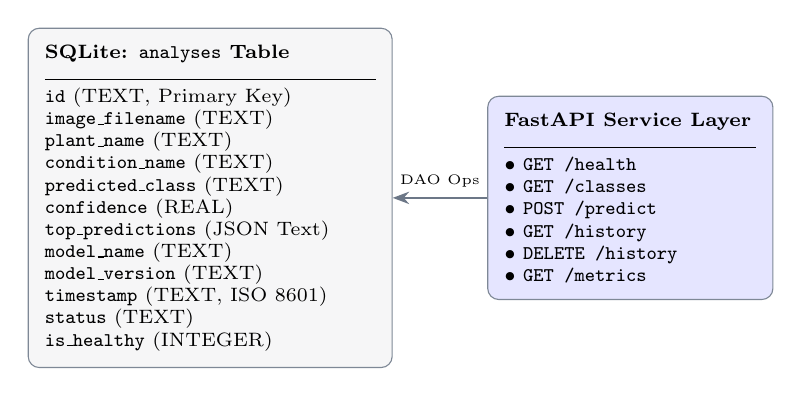
\begin{tikzpicture}[
    box/.style={draw=slate!70, rounded corners=4pt, align=left, font=\scriptsize, inner sep=6pt},
    arrow/.style={-{Stealth[scale=0.9]}, thick, draw=slate!80}
]

\node[box, fill=slate!5] (tbl) {%
    \textbf{SQLite: \texttt{analyses} Table}\\
    \rule{4.2cm}{0.4pt}\\
    \texttt{id} (TEXT, Primary Key)\\
    \texttt{image\_filename} (TEXT)\\
    \texttt{plant\_name} (TEXT)\\
    \texttt{condition\_name} (TEXT)\\
    \texttt{predicted\_class} (TEXT)\\
    \texttt{confidence} (REAL)\\
    \texttt{top\_predictions} (JSON Text)\\
    \texttt{model\_name} (TEXT)\\
    \texttt{model\_version} (TEXT)\\
    \texttt{timestamp} (TEXT, ISO 8601)\\
    \texttt{status} (TEXT)\\
    \texttt{is\_healthy} (INTEGER)
};

\node[box, fill=blue!10, right=1.2cm of tbl] (srv) {%
    \textbf{FastAPI Service Layer}\\
    \rule{3.2cm}{0.4pt}\\
    $\bullet$ \texttt{GET /health}\\
    $\bullet$ \texttt{GET /classes}\\
    $\bullet$ \texttt{POST /predict}\\
    $\bullet$ \texttt{GET /history}\\
    $\bullet$ \texttt{DELETE /history}\\
    $\bullet$ \texttt{GET /metrics}
};

\draw[arrow] (srv) -- node[above, font=\tiny] {DAO Ops} (tbl);

\end{tikzpicture}%
}
\caption{Entity-relationship schema of the persistent SQLite audit database integrated with the FastAPI asynchronous service layer.}
\label{fig:db_schema}
\end{figure}

\subsection{Zero-Simulation Policy}
To preserve academic research validity, BioScan AI implements an absolute zero-simulation guarantee: if model weights are not loaded, the \texttt{POST /predict} endpoint returns an explicit \texttt{HTTP 503 Service Unavailable} status detailing required training actions. The application never generates random predictions or fake outputs.

% ---------------------------------------------------------------------------
% SECTION VIII: DISCUSSION & LIMITATIONS
% ---------------------------------------------------------------------------
\section{Discussion and Real-World Agricultural Constraints}

\subsection{Laboratory vs. In-Situ Field Domain Shift}
A fundamental limitation of public benchmark datasets such as PlantVillage~\cite{hughes2015open} is laboratory background bias: leaves are photographed detached on clean neutral backdrops. In contrast, real-world agricultural scouting entails complex natural backgrounds containing soil, weeds, self-shadowing, dew droplets, and overlapping foliage~\cite{singh2021plantdoc}. Models trained solely on homogeneous backgrounds often learn spurious correlations (e.g., classifying based on background card color rather than lesion morphology).

\subsection{Pathogen Polymorphism and Polymicrobial Complexes}
Field conditions frequently feature co-infections where multiple pathogens simultaneously colonize the same plant (e.g., simultaneous late blight and potato virus Y). Standard multi-class classification assumes mutually exclusive single-label outputs. Future research must expand toward multi-label binary relevance classification and spatial bounding-box localization.

% ---------------------------------------------------------------------------
% SECTION IX: FUTURE EXTENSIONS
% ---------------------------------------------------------------------------
\section{Future Research Roadmap}

The modular architecture of BioScan AI provides a foundation for several advanced biological extensions:
\begin{enumerate}
    \item \textbf{Explainable AI (XAI) Integration:} Implementing Gradient-weighted Class Activation Mapping (Grad-CAM)~\cite{selvaraju2017grad} to produce spatial heatmaps, confirming that neural activations align with true foliar lesions.
    \item \textbf{Cellular Microscopy and Histopathology:} Extending classification to microscopic imagery of stomatal complexes, fungal haustoria penetration, and vascular occlusions.
    \item \textbf{Multi-Modal Telemetry Fusion:} Combining foliar visual features with localized meteorological telemetry (temperature, relative humidity, leaf wetness duration) to predict disease development.
\end{enumerate}

% ---------------------------------------------------------------------------
% SECTION X: CONCLUSION
% ---------------------------------------------------------------------------
\section{Conclusion}
This study presented \textbf{BioScan AI}, an academic experiential-learning system demonstrating reproducible deep learning applied to botanical foliar pathology. By integrating lightweight depthwise separable CNN architectures with strict stratified data partitioning, transparent metric computation, and a decoupled full-stack deployment interface, the system overcomes widespread methodological pitfalls in educational machine learning prototypes. BioScan AI provides a robust foundation for automated plant pathology screening, underscoring the critical distinction between mathematical model confidence and empirical diagnostic truth.

% ---------------------------------------------------------------------------
% ACKNOWLEDGMENT
% ---------------------------------------------------------------------------
\section*{Acknowledgment}
The authors acknowledge the academic guidance of [Course / Faculty Advisor] within the [Academic Department] at [Institution] during the completion of this experiential-learning biological computing research initiative.

% ---------------------------------------------------------------------------
% REFERENCES (inline, no .bib file needed)
% ---------------------------------------------------------------------------
\begin{thebibliography}{99}
\bibitem{fao2021crop} FAO, ``Climate change fans spread of pests and threatens plants and crops,'' Food and Agriculture Organization of the United Nations, 2021.
\bibitem{agrios2005plant} G. N. Agrios, \emph{Plant Pathology}, 5th ed. Academic Press, 2005.
\bibitem{mohanty2016using} S. P. Mohanty, D. P. Hughes, and M. Salath\'e, ``Using deep learning for image-based plant disease detection,'' \emph{Front. Plant Sci.}, vol. 7, p. 1419, 2016.
\bibitem{kamilaris2018deep} A. Kamilaris and F. X. Prenafeta-Bold\'u, ``Deep learning in agriculture: A survey,'' \emph{Comput. Electron. Agric.}, vol. 147, pp. 70--90, 2018.
\bibitem{ferentinos2018deep} K. P. Ferentinos, ``Deep learning models for plant disease detection and diagnosis,'' \emph{Comput. Electron. Agric.}, vol. 145, pp. 311--318, 2018.
\bibitem{guo2017calibration} C. Guo, G. Pleiss, Y. Sun, and K. Q. Weinberger, ``On calibration of modern neural networks,'' in \emph{Proc. ICML}, 2017, pp. 1321--1330.
\bibitem{tiwari2020plant} V. Tiwari, R. C. Joshi, and M. K. Dutta, ``Dense convolutional neural networks based multiclass plant disease detection and classification using leaf images,'' \emph{Ecol. Informatics}, vol. 63, 2021.
\bibitem{barbedo2019plant} J. G. A. Barbedo, ``Plant disease identification from individual lesions and spots using deep learning,'' \emph{Biosyst. Eng.}, vol. 180, pp. 96--107, 2019.
\bibitem{he2016deep} K. He, X. Zhang, S. Ren, and J. Sun, ``Deep residual learning for image recognition,'' in \emph{Proc. CVPR}, 2016, pp. 770--778.
\bibitem{sandler2018mobilenetv2} M. Sandler \emph{et al.}, ``MobileNetV2: Inverted residuals and linear bottlenecks,'' in \emph{Proc. CVPR}, 2018, pp. 4510--4520.
\bibitem{kingma2014adam} D. P. Kingma and J. Ba, ``Adam: A method for stochastic optimization,'' \emph{arXiv:1412.6980}, 2014.
\bibitem{hughes2015open} D. P. Hughes and M. Salath\'e, ``An open access repository of images on plant health to enable the development of mobile disease diagnostics,'' \emph{arXiv:1511.08060}, 2015.
\bibitem{singh2021plantdoc} D. Singh \emph{et al.}, ``PlantDoc: A dataset for visual plant disease detection,'' in \emph{Proc. CoDS-COMAD}, 2020, pp. 249--253.
\bibitem{selvaraju2017grad} R. R. Selvaraju \emph{et al.}, ``Grad-CAM: Visual explanations from deep networks via gradient-based localization,'' in \emph{Proc. ICCV}, 2017, pp. 618--626.
\end{thebibliography}

\end{document}
